\documentclass{rapport}
\usepackage{lipsum}
\usepackage{gensymb}
\usepackage{float}
\usepackage{graphicx} % Required for inserting images
\title{file title} %title of the file

\begin{document}

%----------- Report information ---------

\logo{src/ua_iut_h_couleur_ecran.png}
\uni{\textbf{IUT Angers}}
\ttitle{Projet Drone} %title of the file
\name{nom du drone} % Project Name
\subject{Drone \textit{\name}} % Subject name
\topic{Raport de projet} % Topic name

\professor{M. Yves LETEURTRE \\ 
           M. Xavier PERTHUE}

\students{Simon COUDON\\
          Matéis RAGON} % information related to the students

%----------- Init -------------------
        
\buildmargins % display margins
\buildcover % create the front cover of the document
\toc % creates the table of contents

%------------ Report body ----------------

\section{Introduction}
\subsection{Présentation}
Le projet \textit{\name} est un drone à quatre hélices conçu pour voler et se diriger dans les trois dimensions $(x; y; z)$.

Il possède aussi une embase prévue pour recharger le drone par induction. Il suffit donc de poser le drone sur l'embase et il se recharge. Il possède un témoin lumineux intégré au drone, le premier permet d'indiquer le niveau de la batterie (rouge clignotant si la batterie est faible).

Le drone est équipé d'une caméra, sa vue est retransmise sur le téléphone quand on le pilote. Il est également possible d'enregistrer une vidéo sur le drone. Une carte micro SD est requise pour l'enregistrement de vidéos. Le drone possède également un écran LCD à l'arrière pour écrire le message que l'on souhaite, cette option est disponible dans les paramètres de l'application mobile.

\subsection{Objectif}
L'objectif du drone \textit{\name} est de pouvoir filmer ainsi que de se diriger dans les airs. Il est pilotable par téléphone et peut retransmettre sa vue sur le téléphone qui le commande.

\section{Spécifications techniques}
\subsection{Composants}
La liste des composants ci-dessous est composée du nom du composant ($name$), de la quantité de ce même composant ($qte$), ainsi que la référence produit ($ref$) : 
\begin{table}[htb]
    \centering
    \begin{tabular}{|l|c|r|}
        \hline
        \textbf{QTE} & \textbf{NAME} & \textbf{RÉF} \\
        \hline
        4x & Moteur DC Brushless & $xxx$ \\
        \hline
        1x & NodeMCU - Esp 32 & $xxx$ \\
        \hline
        1x & Capteur Ultrason & $xxx$ \\
        \hline
        1x & Interrupteur ON/OFF & $xxx$ \\
        \hline
        1x & Émetteur induction & $xxx$ \\
        \hline
        1x & Récepteur induction & $xxx$ \\
        \hline
        1x & Batterie $x$V $x$Ah & $xxx$ \\
        \hline
        1x & Support carte micro SD & $xxx$ \\
        \hline
        1x & Caméra & $xxx$ \\
        \hline
        1x & Écran LCD & $xxx$ \\
        \hline
    \end{tabular}
    \caption{Composants}
    \label{tab:my_label}
\end{table}

\subsection{Dimensions}
Les mensurations ci-dessous sont composées du nom de la caractéristique ($name$), ainsi que de sa valeur ($value$) :
\begin{table}[htb]
    \centering
    \begin{tabular}{|l|r|}
        \hline
        \textbf{NAME} & \textbf{VALUE} \\
        \hline
        Longueur (en mm) & $x$ \\
        \hline
        Largeur (en mm) & $x$ \\
        \hline
        Hauteur (en mm) & $x$ \\
        \hline
        Masse (en g) & $x$ \\
        \hline
        ø hélices (en mm) & $x$ \\
        \hline
    \end{tabular}
    \caption{Dimensions}
    \label{tab:my_label}
\end{table}

\subsection{Spécifications électriques}
toto \\

\section{Mouvements}
Pour représenter les moteurs du drone ci-dessous, nous choisissons de prendre une matrice en deux dimensions. Avec chaque élément comme étant un moteur du drone, avec ces coordonnées. \\

{ \centering 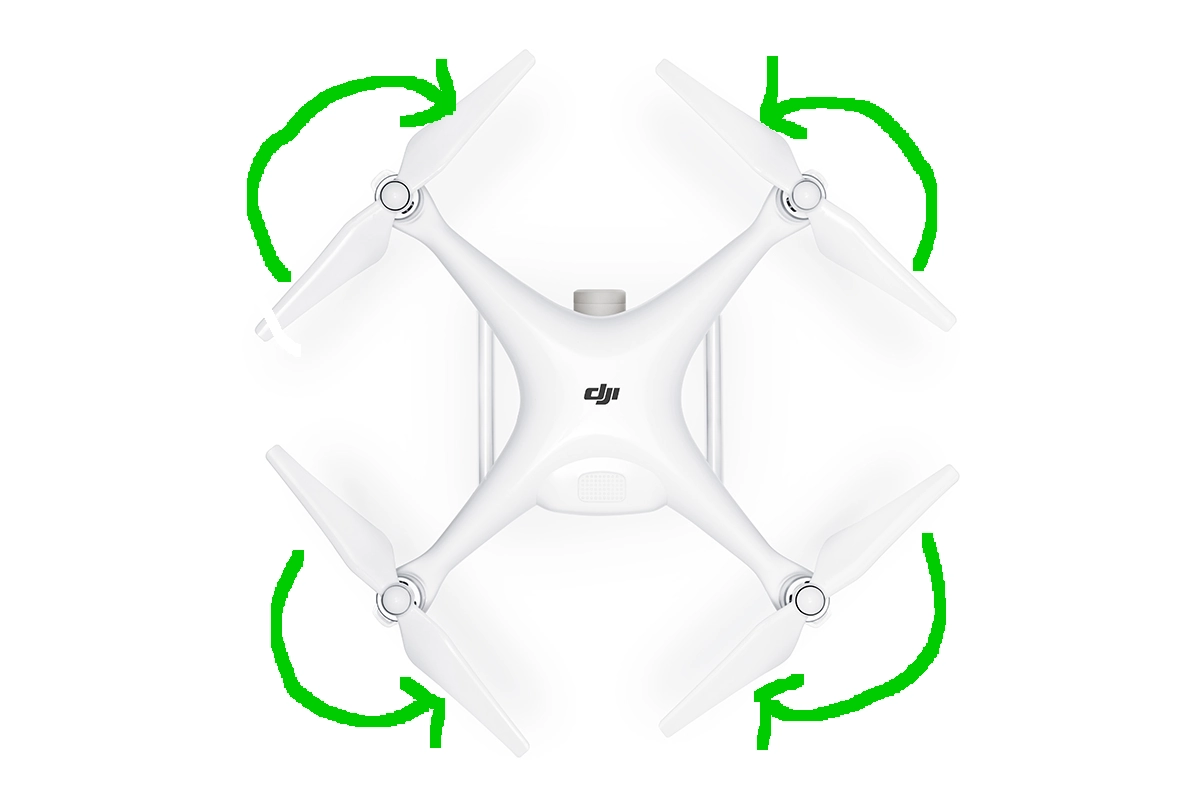
\includegraphics[scale=0.5]{src/1DJI.png} \\}

$$\begin{bmatrix}
(x_1; y_1) & (x_2; y_2) \\
(x_3; y_3) & (x_4; y_4)
\end{bmatrix}$$ \\

Nous nommerons ainsi les moteurs de droite à gauche et de haut en bas, ce qui donne :
$$M_1 = (x_1; y_1)$$
$$M_2 = (x_2; y_2)$$
$$M_3 = (x_3; y_3)$$
$$M_4 = (x_4; y_4)$$

Maintenant, nous pouvons représenter de manière plus concrète les moteurs (les vitesses, sens de rotation, etc.) du drone.

\subsection{Décollage}
Pour l'opération du collage, nous devons respecter un principe simple :

$$ F_z > P_d $$

Avec $F_z$ la force de portance, et $P_d$ le poids du drone, tels que :

$$F_p=\frac{\rho\times V^2 \times S \times C_p}{2}$$

Avec :
\begin{itemize}
    \item $\rho$, la masse volumique de l'air (en $kg \cdot m^{-3}$)
    \item $V^2$, la vitesse du vent (en $m \cdot s^{-1}$)
    \item $S$, la surface de l'air (en $m^2$)
    \item $C_p$, le coefficient de portance (qui dépend de l'angle d'incidence, de la forme de l'aile de l'état de sa surface) \\
\end{itemize}

Sachant que $P_d$ est calculé tel que :

$$\sum m_c \times G$$

Avec :

\begin{itemize}
    \item $m_c$, la masse de tous les composants et de la structure du drone (en $kg$)
    \item $G$, l'intensité de pesanteur (en $N \cdot Kg^{-1}$) \\
\end{itemize}

Ainsi :

$$\frac{\rho\times V^2 \times S \times C_p}{2} > \sum m_c \times G$$

\subsection{Avancer}
Une fois dans les airs, nous devons avancer, pour cela, nous devons augmenter la vitesse des moteurs avant [$M_1; M_2$] et diminuer celles des moteurs arrière [$M_3; M_4$], ce qui nous donne l'équation suivante : \\

$$ V_{M_1M_2} > V_{M_3M_4}$$

Pour cela, nous devons calculer la vitesse individuelle de chaque moteur et la vitesse théorique du drone complet dans différentes situations. \\

Pour calculer la vitesse, nous allons avoir besoins de connaitre la vitesse développée par chaque moteur :

$$ V_m = x $$



\subsection{Reculer}
Pour reculer, c'est l'inverse de l'étape d'avant (avancer), pour cela, nous devons diminuer la vitesse des moteurs avant [$M_1; M_2$] et augmenter celles des moteurs arrière [$M_3; M_4$], ce qui nous donne l'équation suivante : \\

$$ V_{M_1M_2} < V_{M_3M_4}$$

\subsection{Aller à droite}
Pour aller à droite, c'est un peu le même principe que pour avancer ou reculer, il faut diminuer la vitesse des moteurs à droite [$M_1; M_3$] et augmenter celles des moteurs à gauche [$M_2; M_4$], ce qui nous donne l'équation suivante : \\

$$ V_{M_1M_3} < V_{M_2M_4}$$

\subsection{Aller à Gauche}
Pour aller à gauche, c'est l'inverse de l'étape d'avant (aller à droite), il faut augmenter la vitesse des moteurs à droite [$M_1; M_3$] et diminuer celles des moteurs à gauche [$M_2; M_4$]. Ce qui nous donne l'équation suivante : \\

$$ V_{M_1M_3} > V_{M_2M_4}$$

\subsection{Roulis à Droite}
Pour effectuer un roulis à droite, c'est-à-dire une rotation sur la droite, il faut diminuer la vitesse des moteurs dans la diagonale de droite à gauche [$M_1; M_4$], et diminuer la vitesse des moteurs dans la diagonale de gauche à droite [$M_2; M_3$]. Ce qui nous donne l'équation suivante : \\

$$ V_{M_1M_4} > V_{M_2M_3}$$

\subsection{Roulis à Gauche}
Pour le roulis à gauche, on fait l'inverse qu'à droite. On augmente la vitesse des moteurs dans la diagonale de droite à gauche [$M_1; M_4$], et on diminue la vitesse des moteurs dans la diagonale de gauche à droite [$M_2; M_3$]. Ce qui nous donne l'équation suivante :

$$ V_{M_1M_4} < V_{M_2M_3}$$

\section{Montages électroniques}
Nous avons choisi pour mettre tous les composants de faire des PCB (printed circuit board), cela nous procure plusieurs avantages, tout d'abord, une plus grande légèreté, tous composants à mettre directement sur la carte seront en CMS (Composant Monté en Surface). Cela nous assure une plus petite masse totale du drone. Ensuite faire un PCB sur mesure nous permet de relier tous les composants à une seule carte et donc d'avoir le moins de fils dans le boitier. \\

Ainsi pour faire les schémas électroniques, nous avons choisi le logiciel Eagle. Ce logiciel nous permet de faire les schémas et aussi les cartes, pour les imprimer par la suite.

\subsection{Montage de puissance et de commande}
Ce montage correspond à mettre l'$ESP32$, les moteurs, les alimentations à découpage et le connecteur pour la batterie ensemble.

\subsection{Montage des entrées/sorties}
Ce montage consiste à mettre l'$ESP32$, les composants d'entrées/sorties (capteurs, caméra, etc.), la caméra et le support de carte SD.

\subsection{Montage final}
Une fois les montages de puissance, de commande et des entrées/sorties faites, on peut tout rassembler et faire une seule carte, aux dimensions du boitier.

\end{document}
